\subsubsection{Child Deaths vs Socio-Economic Area \& Remoteness}
Successful childbirth often depends on parents' socio-economical status \& geographical location since those determine accessibility to better healthcare, medication better antinatal visiting practices.

In \textbf{Figure \ref{fig:peri_state}} we can see that in Queensland and New South Wales, the perinatal death has always been low but in Northern Territory, it has been high through the years. The graph also shows that neonatal deaths are significantly low in every state through the years compared to stillbirths.
\begin{figure}
  \centering
  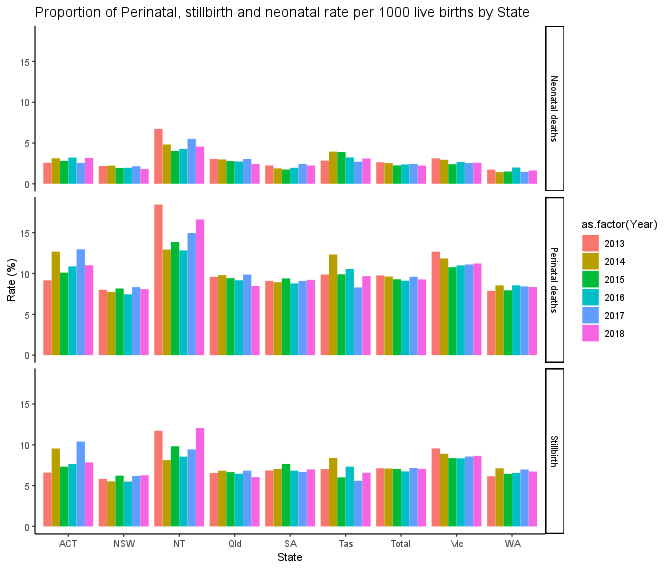
\includegraphics[width=.75\textwidth]{subsections/perinatal_deaths/by_state_birth_baby_death.png}
  \caption{Perinatal death rate per year}
  \label{fig:peri_state}
\end{figure}

To have a deeper understanding, we look into the mother's socio-economic area in \textbf{figure \ref{fig:mother_res}}. Q1 means the most disadvantaged area and Q5 means the least disadvantaged area. It can be clearly observed that the most disadvantaged area has a high mortality rate for all categories of deaths and the least disadvantaged area has the least mortality rate.

\begin{figure}
  \centering
  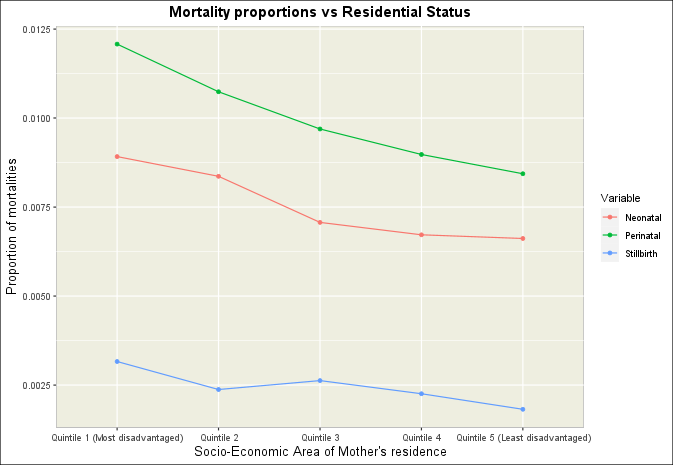
\includegraphics[width=.75\textwidth]{img/aus/kanishka/mortality_residentialStat.png}
  \caption{Socio-economic area of mother's residence}
  \label{fig:mother_res}
\end{figure}

Following that, we wanted to see how the mortality rate was in remote areas in comparison with major cities which are more developed (\textbf{figure \ref{fig:mother_res_remoteness}}). It can be seen that the "Very Remote" areas have the most mortality rate on the other hand major cities have the least death rate.

\begin{figure}
  \centering
  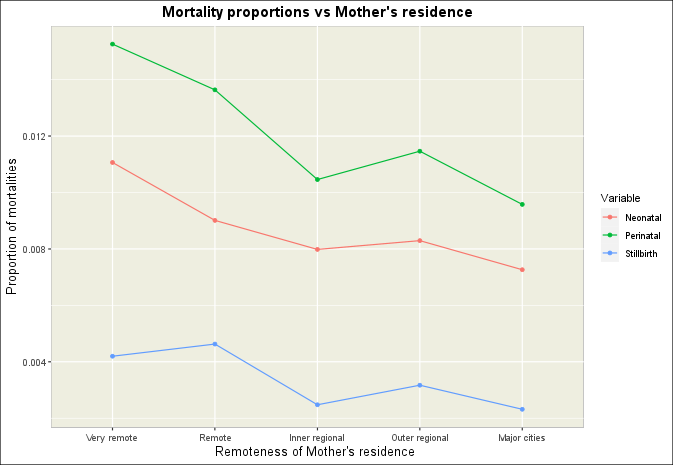
\includegraphics[width=.75\textwidth]{img/aus/kanishka/mortality_mothers_res.png}
  \caption{Remoteness of mother's residence}
  \label{fig:mother_res_remoteness}
\end{figure}